% ============================================================
%  tikz_fig_causal_simple.tex
%  因果推論の根本問題（シンプル版）
%  「政策あり」か「なし」のどちらか一方しか観測できない
% ============================================================
\documentclass[tikz, dvipdfmx]{standalone}
\usepackage{tikz}
\usetikzlibrary{arrows.meta}
\definecolor{gdpblue}{RGB}{30,  90, 180}
\definecolor{obscol} {RGB}{210, 228, 255}   % 観測可能（薄青）
\definecolor{cfcol}  {RGB}{232, 232, 232}   % 観測不可（薄灰）

\begin{document}
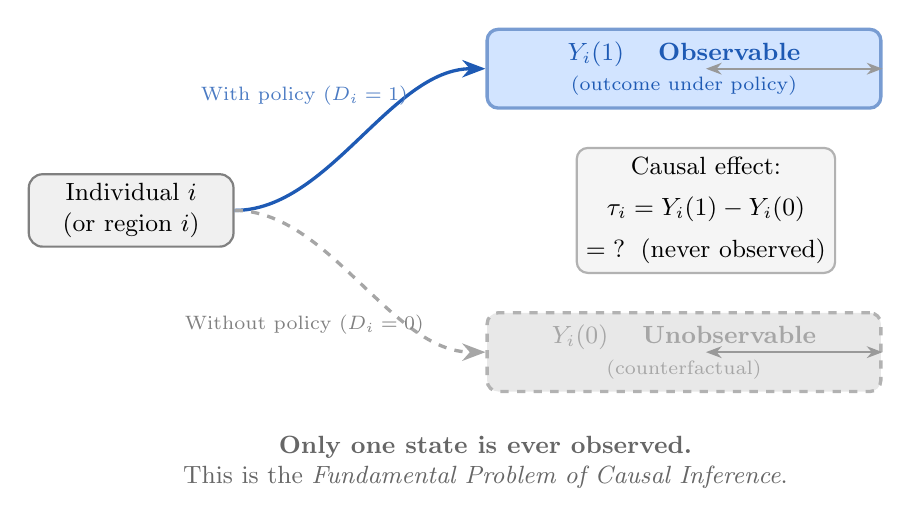
\begin{tikzpicture}[>=Stealth, thick, every node/.style={font=\small}]

% ── 中心ノード（個人 or 地域） ───────────────────────────────
\node[
  draw=black!50, fill=black!6, rounded corners=5pt,
  minimum width=2.6cm, minimum height=0.9cm,
  align=center,
] (unit) at (0,0) {Individual $i$\\(or region $i$)};

% ── 上: 政策あり → 観測可能 ──────────────────────────────────
\draw[->, very thick, gdpblue]
  (unit.east) .. controls +(1.2,0) and +(-1.2,0) .. (4.5, 1.8)
  node[
    draw=gdpblue!60, fill=obscol,
    rounded corners=4pt,
    minimum width=5.0cm, minimum height=1.0cm,
    align=center, anchor=west,
  ] (obs) {$Y_i(1)$ \quad \textbf{Observable}\\
           {\scriptsize (outcome under policy)}};

% 矢印ラベル
\node[font=\scriptsize, gdpblue!80, above] at (2.2, 1.2)
  {With policy ($D_i = 1$)};

% ── 下: 政策なし → 観測不可能 ────────────────────────────────
\draw[->, very thick, dashed, black!35]
  (unit.east) .. controls +(1.2,0) and +(-1.2,0) .. (4.5,-1.8)
  node[
    draw=black!30, fill=cfcol,
    dashed, rounded corners=4pt,
    minimum width=5.0cm, minimum height=1.0cm,
    align=center, anchor=west,
  ] (cf) {$Y_i(0)$ \quad \textbf{Unobservable}\\
          {\scriptsize (counterfactual)}};

% 矢印ラベル
\node[font=\scriptsize, black!50, below] at (2.2,-1.2)
  {Without policy ($D_i = 0$)};

% ── 処置効果の注釈 ───────────────────────────────────────────
\node[
  draw=black!30, fill=black!4, rounded corners=4pt,
  font=\small, align=center,
] at (7.3, 0)
  {Causal effect:\\[4pt]
   $\tau_i = Y_i(1) - Y_i(0)$\\[4pt]
   {\small$= \;?\;$ (never observed)}};

% ── 「どちらか一方しか見えない」矢印 ─────────────────────────
\draw[<->, semithick, black!40]
  (obs.east) -- (7.3, 1.8);
\draw[<->, semithick, black!40]
  (cf.east)  -- (7.3,-1.8);

% ── 下部メッセージ ────────────────────────────────────────────
\node[font=\small, black!60, align=center] at (4.5, -3.2)
  {\textbf{Only one state is ever observed.}\\
   This is the \emph{Fundamental Problem of Causal Inference}.};

\end{tikzpicture}
\end{document}
